\documentclass[letterpaper, 11pt]{extarticle}
% \usepackage{fontspec}

% ==================================================

% document parameters
% \usepackage[spanish, mexico, es-lcroman]{babel}
\usepackage[english]{babel}
\usepackage[margin = 1in]{geometry}

% ==================================================

% Packages for math
\usepackage{mathrsfs}
\usepackage{amsfonts}
\usepackage{amsmath}
\usepackage{amsthm}
\usepackage{amssymb}
\usepackage{physics}
\usepackage{dsfont}
\usepackage{esint}

% ==================================================

% Packages for writing
\usepackage{enumerate}
\usepackage[shortlabels]{enumitem}
\usepackage{framed}
\usepackage{csquotes}

% ==================================================

% Miscellaneous packages
\usepackage{float}
\usepackage{tabularx}
\usepackage{xcolor}
\usepackage{multicol}
\usepackage{subcaption}
\usepackage{caption}
\captionsetup{format = hang, margin = 10pt, font = small, labelfont = bf}

% Citation
\usepackage[round, authoryear]{natbib}

% Hyperlinks setup
\usepackage{hyperref}
\definecolor{links}{rgb}{0.36,0.54,0.66}
\hypersetup{
   colorlinks = true,
    linkcolor = black,
     urlcolor = blue,
    citecolor = blue,
    filecolor = blue,
    pdfauthor = {Author},
     pdftitle = {Title},
   pdfsubject = {subject},
  pdfkeywords = {one, two},
  pdfproducer = {LaTeX},
   pdfcreator = {pdfLaTeX},
   }
\usepackage{titlesec}
\usepackage[many]{tcolorbox}

% Adjust spacing after the chapter title
\titlespacing*{\chapter}{0cm}{-2.0cm}{0.50cm}
\titlespacing*{\section}{0cm}{0.50cm}{0.25cm}

% Indent 
\setlength{\parindent}{0pt}
\setlength{\parskip}{1ex}

% --- Theorems, lemma, corollary, postulate, definition ---
% \numberwithin{equation}{section}

\newtcbtheorem[]{problem}{Problem}%
    {enhanced,
    colback = black!5, %white,
    colbacktitle = black!5,
    coltitle = black,
    boxrule = 0pt,
    frame hidden,
    borderline west = {0.5mm}{0.0mm}{black},
    fonttitle = \bfseries\sffamily,
    breakable,
    before skip = 3ex,
    after skip = 3ex
}{problem}

\tcbuselibrary{skins, breakable}

% --- You can define your own color box. Just copy the previous \newtcbtheorm definition and use the colors of yout liking and the title you want to use.
% --- Basic commands ---
%   Euler's constant
\newcommand{\eu}{\mathrm{e}}

%   Imaginary unit
\newcommand{\im}{\mathrm{i}}

%   Sexagesimal degree symbol
\newcommand{\grado}{\,^{\circ}}

% --- Comandos para álgebra lineal ---
% Matrix transpose
\newcommand{\transpose}[1]{{#1}^{\mathsf{T}}}

%%% Comandos para cálculo
%   Definite integral from -\infty to +\infty
\newcommand{\Int}{\int\limits_{-\infty}^{\infty}}

%   Indefinite integral
\newcommand{\rint}[2]{\int{#1}\dd{#2}}

%  Definite integral
\newcommand{\Rint}[4]{\int\limits_{#1}^{#2}{#3}\dd{#4}}

%   Dot product symbol (use the command \bigcdot)
\makeatletter
\newcommand*\bigcdot{\mathpalette\bigcdot@{.5}}
\newcommand*\bigcdot@[2]{\mathbin{\vcenter{\hbox{\scalebox{#2}{$\m@th#1\bullet$}}}}}
\makeatother

%   Hamiltonian
\newcommand{\Ham}{\hat{\mathcal{H}}}

%   Trace
\renewcommand{\Tr}{\mathrm{Tr}}

% Christoffel symbol of the second kind
\newcommand{\christoffelsecond}[4]{\dfrac{1}{2}g^{#3 #4}(\partial_{#1} g_{#2 #4} + \partial_{#2} g_{#1 #4} - \partial_{#4} g_{#1 #2})}

% Riemann curvature tensor
\newcommand{\riemanncurvature}[5]{\partial_{#3} \Gamma_{#4 #2}^{#1} - \partial_{#4} \Gamma_{#3 #2}^{#1} + \Gamma_{#3 #5}^{#1} \Gamma_{#4 #2}^{#5} - \Gamma_{#4 #5}^{#1} \Gamma_{#3 #2}^{#5}}

% Covariant Riemann curvature tensor
\newcommand{\covariantriemanncurvature}[5]{g_{#1 #5} R^{#5}{}_{#2 #3 #4}}

% Ricci tensor
\newcommand{\riccitensor}[5]{g_{#1 #5} R^{#5}{}_{#2 #3 #4}}
\usepackage{physics}
\usepackage{quantikz} % Ensure this is present
\usepackage{tikz}
\usetikzlibrary{quantikz2}
\usepackage{amsmath}
\usepackage{amssymb}
\usetikzlibrary{arrows.meta}
\begin{document}

\begin{Large}
    \textsf{\textbf{Assignment 1 Fundamentals}}
    
    Quantum Information Systems
\end{Large}

\vspace{1ex}

\textsf{\textbf{Student:}} \text{Jesus R. Lopez}, \href{mailto:jlopez126@miners.utep.edu}{\texttt{jlopez126@miners.utep.edu}}\\
\textsf{\textbf{Lecturer:}} \text{Mohammad Saidur Rahman}, \href{mailto:msrahman3@utep.edu}{\texttt{msrahman3@utep.edu}}


\vspace{2ex}

This book was used as a reference to solve these problems \cite{Wong2022}

\begin{problem}{Solve}{problem-label}
Determine if each pair of states is orthogonal or not.

First let us recall the following:

Two quantum states $\ket{\psi}$ and $\ket{\phi}$ are ortogonal if their inner product is zero:
\[
\langle  \;\psi | \phi \; \rangle = 0
\]

\begin{enumerate}[(a)]
    \item $\ket{+}$  and $\ket{-}$\\
   	\textbf{Answer:}\\
   	The Hadamard basis states are:
   	\[
   	\ket{+} = \frac{1}{\sqrt{2}} (\ket{0}+\ket{1}),  \ket{-} = \frac{1}{\sqrt{2}} (\ket{0}-\ket{1})
   	\]
   	Their inner product is:
   	\[
   	\langle + \; | \; - \rangle = (\frac{1}{\sqrt{2}} (\bra{0}+\bra{1})) (\frac{1}{\sqrt{2}} (\ket{0}-\ket{1}))
   	\]
   	Distributing:
   	\[
   	= \frac{1}{2} (\langle 0 | 0\rangle  - \langle 0 | 1\rangle  + \langle 1 | 0\rangle - \langle 0 | 1\rangle)
   	\]
   	
   	Final results
   	\[
	= \frac{1}{2}(1-0+0-1) = \frac{1}{2} (1-1) = 0
	\]
	\textbf{Conclusion} is orthogonal
    \item  $\ket{0}$ and $\ket{+}$ \\
    \textbf{Answer:}\\
    Now $\ket{0} is$:
    \[
    \ket{0}=
    \begin{bmatrix}
    	1\\
    	0
    \end{bmatrix}
    \]
   $\ket{+} is$:
   \[
   \ket{+} = \frac{1}{\sqrt{2}} 
   \begin{bmatrix}
   	1\\
   	1
   \end{bmatrix}
   \]
   
    Now let us compute the inner product $\langle 0 | + \rangle$:\\
    \[
    \bra{0} = 
    \begin{bmatrix}
    	1 & 0
    \end{bmatrix} 
    and 
     \ket{+} = \frac{1}{\sqrt{2}} 
    \begin{bmatrix}
    	1\\
    	1
    \end{bmatrix}
    \]
    So, 
    \[
    \langle 0 | + \rangle = (
    \begin{bmatrix}
    	1 & 0
    \end{bmatrix} 
    )(\frac{1}{\sqrt{2}} 
    \begin{bmatrix}
    	1\\
    	1
    \end{bmatrix}
    )\]
    Multiplying the row vector by the column vector:
    \[
     \langle 0 | + \rangle = \frac{1}{\sqrt{2}} 
     \begin{bmatrix}
     	1 * 1+ 0*1
     \end{bmatrix} = 
     \frac{1}{\sqrt{2}} (1 + 0) = \frac{1}{\sqrt{2}}
    \]
    \textbf{Conclusion}: not orthogonal
    
	\item $
	\frac{1+\sqrt{3}i}{4} \ket{0} + \frac{\sqrt{2}-i}{2} \ket{1} \quad \text{and} \quad \frac{\sqrt{2}+i}{2} \ket{0} + \frac{-1+\sqrt{3}i}{4} \ket{1}.
	$\\
    \textbf{Answer:}\\
    The first part we are going to call it:
    \[
    \ket{\psi} = \frac{1+\sqrt{3}i}{4} \ket{0} + \frac{\sqrt{2}-i}{2} \ket{1} \quad
    \]
    The second part we are going to call it:
    \[
    \ket{\phi} = \frac{\sqrt{2}+i}{2} \ket{0} + \frac{-1+\sqrt{3}i}{4} \ket{1}.
    \]
   first we have to calculate $ \bra{\psi}$, which in vector form its easier to understand:
    \[
    \ket{\psi} = \begin{bmatrix*}
    	\frac{1+\sqrt{3}i}{4}\\
    	\frac{\sqrt{2}-i}{2} 
    \end{bmatrix*}
    \]
    \[
    \bra{\psi} = 
    \begin{bmatrix}
    	\frac{1-\sqrt{3}i}{4} & \frac{\sqrt{2}+i}{2} 
    \end{bmatrix}
    \]
     From here we want to calculate the inner product:
    \[
    \langle \psi | \phi \rangle
    \]
    we are going to take the ones from the combination of $\langle 0 | 0 \rangle$ and $\langle 1 | 1 \rangle$ because the other combinations will yield to 0.
    \[
    \langle \psi | \phi \rangle = \frac{1-\sqrt{3}i}{4} *  \frac{\sqrt{2}+i}{2}  +  \frac{\sqrt{2}+i}{2} * \frac{-1+\sqrt{3}i}{4}
    \]
    doing linear algebra we are going to get:
    \[
      \langle \psi | \phi \rangle = \frac{0}{8} + \frac{0}{8} = 0
    \]
    
    
    \textbf{Conclusion}: Orthogonal
\end{enumerate}
\end{problem}



\begin{problem}{Proof.}{problem-label-2}
\begin{enumerate}[(a)]
    \item  Show that the Hadamard gate is unitary by computing $H^{\dagger} H$
\end{enumerate}
\textbf{Answer:}\\
	First lets start by recalling what is the definition of a unitary matrix:\\

\[
U^{\dagger}U = I
\]

where $U^{\dagger}$ is the hermitian transpose of U, and I is the identity of the matrix. Now, the Hadamard gate matrix is:
\[
H =\frac{1}{\sqrt{2}} 
\begin{bmatrix}
	1 & 1\\
	1 & -1
\end{bmatrix}
\]
Now, let us do the Hermitian Adjoint, which is simply its transpose:
\[
H^{\dagger}= \frac{1}{\sqrt{2}}
\begin{bmatrix}
	1 & 1\\
	1 & -1
\end{bmatrix}
\]
Now we are going to compute $H^{\dagger}H$
\[
H^{\dagger}H =
\frac{1}{\sqrt{2}}
\begin{bmatrix}
	1 & 1\\
	1 & -1
\end{bmatrix}
*
\frac{1}{\sqrt{2}}
\begin{bmatrix}
	1 & 1\\
	1 & -1
\end{bmatrix}
\]

\[
H^{\dagger}H = \frac{1}{2}
\begin{bmatrix}
	(1*1+1*1) & (1*1+-1*1)\\
	(1*1+1*-1) & (1*1+-1*-1)
\end{bmatrix}
= \frac{1}{2}
\begin{bmatrix}
	2 & 0 \\
	0 & 2
\end{bmatrix}
= 
\begin{bmatrix}
	1 & 0 \\
	0 & 1
\end{bmatrix}
= I 
\]








\end{problem}


\begin{problem}{ Proof.}{problem-label-3}
	
	\begin{enumerate}[(a)]
		\item Prove that Pauli X matrix is unitary
	\end{enumerate}
	\textbf{Answer:}\\
	First lets start by recalling what is the definition of a unitary matrix:\\
	
	\[
	U^{\dagger}U = I
	\]
	
	where $U^{\dagger}$ is the hermitian transpose of U, and I is the identity of the matrix. Now, the Pauli X matrix is:
	\[
	X = 
	\begin{bmatrix}
		0 & 1\\
		1 & 0
	\end{bmatrix}
	\]
	Now, let us do the Hermitian Adjoint, which is simply its transpose:
	\[
	X^{\dagger}= 
	\begin{bmatrix}
		0 & 1\\
		1 & 0
	\end{bmatrix}
	\]
	Now, we are going to compute $X^{\dagger}X$:
	\[
	X^{\dagger}X = 
	\begin{bmatrix}
		0 & 1\\
		1 & 0
	\end{bmatrix}
	*
	\begin{bmatrix}
		0 & 1\\
		1 & 0
	\end{bmatrix}
	\]
	
	\[
	X^{\dagger}X = 
	\begin{bmatrix}
		(0*0 + 1*1) & (0*1+1*0)\\
		(1*0+0*1)& (1*1+0*0)
	\end{bmatrix}
	=
	\begin{bmatrix}
		1 & 0\\
		0 & 1
	\end{bmatrix}
	= I
	\]
	
\end{problem}

\begin{problem}{Bell State }{problem-label-4}
	
	\begin{enumerate}[(a)]
		\item Show that the bell state is entangled by proving that it cannot be written as a product state $\ket{\Psi^+}$.
	\end{enumerate}
	\textbf{Answer:}
	our goal is to prove that we cannot  write a bell state as a product state. 
	
	for this problem we know that:
	
	\[
	\ket{\Psi^+} = \frac{1}{\sqrt{2}} (\ket{01}+\ket{10})
	\]
	
	Well, First we are going to start to write it as a product state:\\
	\[
	\begin{aligned}
		\ket{\Psi_A} &= \alpha\ket{0} + \beta\ket{1} \\
		\ket{\Psi_B} &= \gamma\ket{0} + \delta\ket{1} \\
		\ket{\Psi^+} &= \ket{\Psi_A} \otimes \ket{\Psi_B}\\\\
	\end{aligned}
	\]
	Where $\alpha,\beta,\gamma,\delta$ are complex numbers satisfying normalization:
	\[
	\begin{aligned}
		\abs{\alpha}^2 + \abs{\beta}^2 &= 1\\
		\abs{\gamma}^2 + \abs{\delta}^2 &= 1
	\end{aligned}
	\]
	Now, let us do the product (tensor) state operation:
	\[
	\begin{aligned}
		\ket{\Psi_A} \otimes \ket{\Psi_B} &=   \alpha\gamma\ket{00} + \alpha\delta\ket{01} + \beta\gamma\ket{10} +  \beta\delta\ket{11}
	\end{aligned}
	\]
	It is time to match the coefficients:
	\[
	\begin{aligned}
		\alpha\gamma &= 0\\
		\beta\delta &= 0 \\
		\alpha\delta &= \frac{1}{\sqrt{2}}\\
		\beta\gamma &= \frac{1}{\sqrt{2}}
	\end{aligned}
	\]
	Now, we can set the the coefficients of $\ket{00} and \ket{11}$ to 0 becuase we do not need them, but being equal to 0 means that either $ \alpha$ or $\gamma$ and $\beta$ or $\delta$ is 0. \\
	
	\textbf{Contradiction:} the problem is the following:
	\begin{itemize}
		\item if $\alpha = 0$, then $\alpha\delta \not= \frac{1}{2}$
		\item if $\gamma = 0$, then $\beta\gamma \not= \frac{1}{2}$
		\item if $\delta = 0$, then $\alpha\delta \not= \frac{1}{2}$
		\item if $\beta = 0$, then $\beta\gamma \not= \frac{1}{2}$
	\end{itemize}
	
	From this we can \textbf{conclude} that it is entangled because the states are not separated and cannot be represented as a tensor product due the contradiction stated before.
\end{problem}

\begin{problem}{Quantum Circuit }{problem-label-5}
	
	\begin{enumerate}[(a)]
		\item Construct a quantum circuit to generate a bell state $\ket{\Psi^-}$
	\end{enumerate}
	\textbf{Answer:}\\
\[
	\begin{quantikz}
	q_0 &\gate{x}&\gate{H}&\ctrl{1}&& \\
	q_1 &\gate{x}&&\targ{}&&
\end{quantikz}
\]
Why does this makes sense?

First we start with:

\[
q_0 = \ket{0} 
\]
By applying Pauli-X we get :

\[
X\ket{0}=\ket{1}
\]
after appplying Hadamar we get:

\[
H\ket{1} = \frac{\ket{0}-\ket{1}}{\sqrt{2}}
\]
On the other hand, for $q_1$ we are going to apply Pauli-X:

\[
q_1 = \ket{0}
\]

Then:

\[
\frac{\ket{0}-\ket{1}}{\sqrt{2}} \ket{1}
\]

\[
\frac{\ket{01}-\ket{11}}{\sqrt{2}} 
\]

Because:

\[
\ket{q_0 q_1}
\]

Finally we apply the control gate and we got :

\[
\frac{\ket{01}-\ket{10}}{\sqrt{2}} = \ket{\Psi^-} 
\]
\end{problem}

\newpage%removeeeeeee
\begin{problem}{GHZ}{problem-label-6}
	
	\begin{enumerate}[(a)]
		\item Construct a three-qubit GHZ state and show that measuring any qubit collapses the entire system.
	\end{enumerate}
	\textbf{Answer:}\\
	a three-qubit GHZ state is in the following form:
	\[
	\ket{GHZ} = \frac{1}{\sqrt{2}}(\ket{000}+\ket{111})
	\]
	So we start with three qubits in the state $\ket{0}$:
	\[
	\ket{\psi_0} = \ket{000}
	\]
	This can be represented as 
	\[
	\ket{0}\otimes\ket{0}\otimes\ket{0}
	\]
	From here we are going to apply Hadamar to the first qubit:
	\[
	\ket{\psi_o} = \textit{H}\ket{0} \otimes \ket{0}\otimes\ket{0}
	\]
	\[
	\ket{\psi_o} = \frac{1}{\sqrt{2}}(\ket{0} + \ket{1}) \otimes \ket{0}\otimes\ket{0}
	\]
	Then 
	\[
	= \frac{1}{\sqrt{2}} (\ket{000}+ \ket{100})
	\]
	from here we are going to apply control gates, the first one is going to be the contriol and the second one is going to be the target:
	\[
	Cnot_{1->2}\ket{\psi_0} = \frac{1}{\sqrt{2}} (\ket{000}+ \ket{110})
	\]
	then we are going to apply cnot again and the control is 1 and the target is 3:
	\[
		Cnot_{1->3}\ket{\psi_0} = \frac{1}{\sqrt{2}} (\ket{000}+ \ket{111}) = \ket{GHZ}
	\]
	
	Now, if we expand it to:
	\[
	\ket{GHZ} = \frac{1}{\sqrt{2}} (\ket{0}\otimes\ket{00}+\ket{1}\otimes\ket{11})
	\]
	The first qubit is in superposition  $\ket{0}$ and $\ket{1}$, and we know that the probabilities of measuring $\ket{0}$ is $\frac{1}{2}$ and the same applies to $\ket{1}$.
	
	If we measure the first qubit and get a 0, the state collapses to $ \ket{0}\otimes\ket{00}$ or $\ket{000}$. This merans that all three qubits are now in the state $\ket{000}$
	
	\textbf{Why does it happen?} Well, the quibits are entangles, measuring one of them instantly determins the state of all the others.

\end{problem}

\begin{problem}{CNOT}{problem-label-7}
	
	\begin{enumerate}[(a)]
		\item Explain the role of the CNOT gate in entanglement creation and provide a mathematial proof.
	\end{enumerate}
	\textbf{Answer:}\\
	We will begin with the bell state by first doing hadamard:
	\[
	\ket{\psi_0} = \ket{0} \otimes \ket{0} = \ket{00}
	\]
	\[
	H\ket{0} = \frac{1}{\sqrt{2}} (\ket{0}+\ket{1})
	\]
	Now following the system transform into:
	\[
	= \frac{1}{\sqrt{2}} (\ket{0}+\ket{1}) \otimes \ket{0}
	\]
	\[
	= \frac{1}{\sqrt{2}} (\ket{00}+\ket{10})
	\]
	Now, we are going to apply the CNOT gate and we have to remember that the first qubit works as the control and the second as the target, in the end we get:
		\[
	= \frac{1}{\sqrt{2}} (\ket{00}+\ket{11}) = \ket{\Phi^+}
	\]
	
	We know from previous proofs that the bell states such as :
	\[
	\ket{\Phi^+} = \frac{1}{\sqrt{2}} (\ket{00}+ \ket{11})
	\]
	cannot be represented with tensor products because states cannot be separated and we tend to run into a contradiction, therefore there is entanglement.
\end{problem}


\begin{problem}{Quantum Circuit}{problem-label-8}
	
	\begin{enumerate}[(a)]
		\item Construct a quantum circuit that applies an X gate followed by a Hadamard gate on a single qubit. what does the qubit end in?
	\end{enumerate}
	\textbf{Answer:}
	
	\[
	\begin{quantikz}
		q_0 &\gate{x}&\gate{H}&
	\end{quantikz}
	\]
	Now, lets trace que qubit:
	
	$q_0 = \ket{0}$
	
	Then we apply Pauli-X:
	
	$X\ket{0} = \ket{1}$
	
	Finally, we apply Hadamard gate:
	
	$H\ket{1} =  \frac{\ket{0}-\ket{1}}{\sqrt{2}} $
	
\end{problem}

For the next problem I changed $\ket{\Psi^+} to \ket{\Psi^-} $, just to experiment
\begin{problem}{Bell States}{problem-label-9}
	
	\begin{enumerate}[(a)]
		\item Show that the bell state is entangled by proving that it cannot be written as a product state $\ket{\Psi^-}$.
	\end{enumerate}
	\textbf{Answer:}
	
	our goal is to prove that we cannot  write a bell state as a product state. 
	
	for this problem we know that:
	
	\[
	\ket{\Psi^-} = \frac{1}{\sqrt{2}} (\ket{01}-\ket{10})
	\]
	
	Well, First we are going to start to write it as a product state:\\
		\[
		\begin{aligned}
			\ket{\Psi_A} &= \alpha\ket{0} + \beta\ket{1} \\
			\ket{\Psi_B} &= \gamma\ket{0} + \delta\ket{1} \\
			\ket{\Psi^-} &= \ket{\Psi_A} \otimes \ket{\Psi_B}\\\\
		\end{aligned}
		\]
		Where $\alpha,\beta,\gamma,\delta$ are complex numbers satisfying normalization:
		\[
		\begin{aligned}
		\abs{\alpha}^2 + \abs{\beta}^2 &= 1\\
		\abs{\gamma}^2 + \abs{\delta}^2 &= 1
		\end{aligned}
		\]
		Now, let us do the product (tensor) state operation:
		\[
		\begin{aligned}
			 \ket{\Psi_A} \otimes \ket{\Psi_B} &=   \alpha\gamma\ket{00} + \alpha\delta\ket{01} + \beta\gamma\ket{10} +  \beta\delta\ket{11}
		\end{aligned}
		\]
		It is time to match the coefficients:
		\[
		\begin{aligned}
			 \alpha\gamma &= 0\\
			 \beta\delta &= 0 \\
			 \alpha\delta &= \frac{1}{\sqrt{2}}\\
			 \beta\gamma &= - \frac{1}{\sqrt{2}}
		\end{aligned}
		\]
		Now, we can set the the coefficients of $\ket{00} and \ket{11}$ to 0 becuase we do not need them, but being equal to 0 means that either $ \alpha$ or $\gamma$ and $\beta$ or $\delta$ is 0. \\
		
	\textbf{Contradiction:} the problem is the following:
	\begin{itemize}
		\item if $\alpha = 0$, then $\alpha\delta \not= \frac{1}{2}$
		\item if $\gamma = 0$, then $\beta\gamma \not= -\frac{1}{2}$
		\item if $\delta = 0$, then $\alpha\delta \not= \frac{1}{2}$
		\item if $\beta = 0$, then $\beta\gamma \not= -\frac{1}{2}$
	\end{itemize}
		
			From this we can \textbf{conclude} that it is entangled because the states are not separated and cannot be represented as a tensor product due the contradiction stated before.
\end{problem}

For the following problem it was not required to answer but I wanted to introduce the algorithm by paper and also by code.
\begin{problem}{Quantum Circuit}{problem-label-10}
	
	\begin{enumerate}[(a)]
		\item Implement a Quantum Circuit for the Deutsh-Josza algorithm and verify its operation.
	\end{enumerate}
	\textbf{Answer:}
	Well, Lets say we are given a algorithm \textit{f(x)} that takes one bit \textit{x} as an input and returns one bit f(x)
	
	
\[
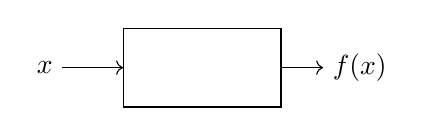
\begin{tikzpicture}[node distance=2cm, auto]
 %Nodes
	\node (input) {$x$};
	\node[draw, rectangle, minimum width=2cm, minimum height=1cm, right of=input] (blackbox) {};
	\node[right of=blackbox] (output) {$f(x)$};
	% Arrows
	\draw[-> ] (input) -- (blackbox);
	\draw[-> ] (blackbox) -- (output);
\end{tikzpicture}
\]
We need to check whether the result actually depends on the input or not. As mentions \cite{Kosheleva2021} mentions, one example for this algorithm is the weather prediction in El Paso, To predict tomorrows weather we can use today's weather data from all over the world. However, in reality only weather in the small vicinty of El Paso is relevant. These kind of problems are important because as mentioned, weather prediction is a good example of a program f that requires a lot of computations, but it is important to solve the probelm with few calls to the program f as possible.\\


\textbf{Deutsch-Jozsa Algorithm}
\begin{itemize}[]
	\item First, We start with the state $\ket{0,1}$ = $\ket{0}\otimes\ket{1}$
	\item We apply the Hadamard Transformation \textit{H} to Both Bits
	\item Then, we apply \textit{f}
	\item After that, we again apply the Hadamard transformation to both bits:
	\begin{itemize}[]
		\item If the first bit is 0, we conclude that the function \textit{f} is constant.
		\item If the first bit is 1, we conclude that hte function is not constant.
		\end{itemize}
\end{itemize}
\textbf{Example:}\\

We start with $\ket{0,1}$, then we expand it and apply Hadamard transformations.

\[
H\ket{0} \otimes H\ket{1} = (\frac{1}{\sqrt{2}}\ket{0} + \frac{1}{\sqrt{2}}\ket{1}) \otimes (\frac{1}{\sqrt{2}}\ket{0}-\frac{1}{\sqrt{2}}\ket{1})
\]
We distribute and we get:
\[
H\ket{0} \otimes H\ket{1} = \frac{1}{\sqrt{2}}\ket{00}- \frac{1}{\sqrt{2}}\ket{01} + \frac{1}{\sqrt{2}}\ket{10}-\frac{1}{\sqrt{2}}\ket{11}
\]
What happens next, depends on the function \textit{f}. The left numbers of the table is corresponding for f(1) and the numbers on the top is corresponding for f(0).
\[
\begin{array}{c|c|c}
	 & 0 & 1 \\ \hline
	0 & F(x) = 0 & F(x) = !x \\
	1 & F(x) = x & F(x) = 1
\end{array}
\]
\[
\textit{f}(x,y) -> \ket{x,y\otimes \textit{f}(x)}
\]
for \textit{f}(x) = 1
\[
\ket{x,y} -> \ket{x,y\otimes1} 
\]
\[
\ket{0,0} -> \ket{0,0\otimes1} = \ket{0,1}
\]
\[
\ket{0,1} -> \ket{0,1\otimes1} = \ket{0,0}
\]
\[
\ket{1,0} -> \ket{1,0\otimes1} = \ket{1,1}
\]
\[
\ket{1,1} -> \ket{1,1\otimes1} = \ket{1,0}
\]

\[
\frac{1}{2} \ket{01} -\frac{1}{2}\ket{00}+\frac{1}{2}\ket{11}-\frac{1}{2}\ket{10}=
\]
\[
=\frac{1}{2} \ket{0}\otimes\ket{1} -\frac{1}{2}\ket{0}\otimes\ket{0}+
\frac{1}{2}\ket{1}\otimes\ket{1}-\frac{1}{2}\ket{1}\otimes\ket{0}=
\]
\[
=\frac{1}{\sqrt{2}}\ket{0}\otimes(\ket{1}-\ket{0})+\frac{1}{\sqrt{2}}\ket{1}\otimes(\ket{1}-\ket{0})=
\]
\[
=(\frac{1}{\sqrt{2}}\ket{0} + \frac{1}{\sqrt{2}}\ket{1}) \otimes (\frac{1}{\sqrt{2}}\ket{0}-\frac{1}{\sqrt{2}}\ket{1})=
\]
\[
-\ket{0} \otimes \ket{1}
\]

\end{problem}




% =================================================

\newpage
\vfill
\bibliographystyle{apalike}
\bibliography{references}

\end{document}